\documentclass[tikz,border=2pt]{standalone}
\usepackage[utf8]{inputenc}
% Glyphs shared by all element diagrams of the plate bending demo
\tikzset{
    cell/.style={draw=black, thick},
    edge dof/.style={->, ultra thick, black},
    operator/.style={->, very thick, black},
}
\newcommand{\scalardof}[1]{\fill[black] #1 circle (2pt);}
\newcommand{\vectordof}[1]{\fill[black] #1 ++(-0.08,0) circle (2pt); \fill[black] #1 ++(0.08,0) circle (2pt);}
\newcommand{\gradientdof}[1]{\draw[black, thick] #1 circle (4pt);}
\begin{document}
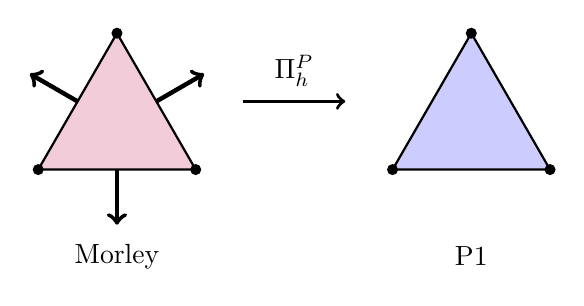
\begin{tikzpicture}

    % Morley element: vertex values and normal derivatives on the edges
    \begin{scope}[shift={(0,0)}]
        \filldraw[fill=purple!20, cell] (0,0) -- (2,0) -- (1,1.732) -- cycle;
        \draw[edge dof] (1,0) -- (1,-0.7);
        \draw[edge dof] (1.5,0.866) -- (2.106,1.216);
        \draw[edge dof] (0.5,0.866) -- (-0.106,1.216);
        \foreach \p in {(0,0), (2,0), (1,1.732)} {\scalardof{\p}}
        \node at (1,-1.1) {Morley};
    \end{scope}

    % Reduction operator
    \draw[operator] (2.6,0.866) -- (3.9,0.866);
    \node at (3.25,1.25) {$\Pi_h^P$};

    % P1 element: vertex values
    \begin{scope}[shift={(4.5,0)}]
        \filldraw[fill=blue!20, cell] (0,0) -- (2,0) -- (1,1.732) -- cycle;
        \foreach \p in {(0,0), (2,0), (1,1.732)} {\scalardof{\p}}
        \node at (1,-1.1) {P1};
    \end{scope}

\end{tikzpicture}
\end{document}
